\section{Experimental data and setup}
\label{sec:experiments}
The phoneme representations in each layer are calculated as the
activations averaged over the duration of the phoneme occurrence in the
input. The average input vectors are similarly calculated as the MFCC
vectors averaged over the time course of the articulation of the
phoneme occurrence. When we need to represent a phoneme type we do so by
averaging the vectors of all its occurrences in the validation set.
\begin{table}[t]
  \centering
  \begin{tabular}{l|c}
    Vowels & \textipa{i I U u}\\
           & \textipa{e E \textschwa{} \textrhookschwa{} OI O o }
             \\
           & \textipa{aI \ae{} \textturnv{} \textscripta{}  aU }\\
    Approximants & \textipa{j \textturnr{} l w }\\
    Nasals      & \textipa{m n N } \\
    Plosives   & \textipa{p  b  t  d  k  g }\\
    Fricatives & \textipa{f v T \dh{} s z S Z h }\\
    Affricates & \textipa{\textteshlig{} \textdyoghlig{} }\\
  \end{tabular}
  \caption{Phonemes of General American English.}
  \label{tab:phoneme-list}
\end{table}
Table~\ref{tab:phoneme-list} shows the phoneme inventory we work with; this is also the inventory used by Gentle/Kaldi (see Section~\ref{sec:forced}).


\subsection{Model settings}
\label{sec:parameters}
We use the pre-trained version of the COCO~Speech model, implemented
in Theano \citep{Bastien-Theano-2012}, provided by
\citet{chrupala2017representations}.\footnote{Code, data and
  pretrained models available from \href{https://github.com/gchrupala/visually-grounded-speech}{https://github.com/gchrupala/visually-grounded-speech}.}
The details of the model configuration are as follows: convolutional
layer with length 6, size 64, stride 3, 5 Recurrent Highway Network
layers with 512 dimensions and 2 microsteps, attention Multi-Layer
Perceptron with 512 hidden units, Adam optimizer, initial learning
rate 0.0002. The 4096-dimensional image feature vectors come from the
final fully connect layer of VGG-16 \citep{simonyan2014very}
pre-trained on Imagenet \cite{ILSVRCarxiv14}, and are averages of
feature vectors for ten crops of each image.  The total number of
learnable parameters is 9,784,193. Table~\ref{tab:arch} sketches the
architecture of the utterance encoder part of the model.

\begin{table}[t]
  \centering
  \begin{tabular}{|c|}\hline
    Attention: size 512 \\\hline
    Recurrent 5: size 512 \\\hline
    Recurrent 4: size 512 \\\hline
    Recurrent 3: size 512 \\\hline
    Recurrent 2: size 512 \\\hline
    Recurrent 1: size 512 \\\hline
    Convolutional: size 64, length 6, stride 3 \\\hline\hline
    Input MFCC: size 13 \\\hline
  \end{tabular}
  \caption{COCO~Speech utterance encoder architecture.}
  \label{tab:arch}
\end{table}

\subsection{Synthetically Spoken COCO}
\label{sec:coco}
The Speech~COCO model was trained on the Synthetically Spoken COCO dataset \citep{grzegorz_chrupala_2017_400926}, which is a version of the MS~COCO dataset \citep{lin2014microsoft} where speech was synthesized for the original image descriptions, using high-quality speech synthesis provided by gTTS.\footnote{Available at \href{https://github.com/pndurette/gTTS}{https://github.com/pndurette/gTTS}.}

\subsection{Forced alignment}
\label{sec:forced}
We aligned the speech signal to the corresponding phonemic transcription with the Gentle toolkit,\footnote{Available at
  \href{https://github.com/lowerquality/gentle}{https://github.com/lowerquality/gentle}.}
which in turn is based on Kaldi \citep{Povey_ASRU2011}. It 
uses a speech recognition model for English to transcribe the input audio
signal, and then finds the optimal alignment of the transcription to
the signal. This fails for a small number of utterances, which we
remove from the data.  In the next step we extract MFCC features from
the audio signal and pass them through the COCO~Speech utterance encoder, and
record the activations for the convolutional layer as well as all the
recurrent layers. For each utterance the representations (i.e.\ MFCC
features and activations) are stored in a $t_r\times D_r$ matrix, where
$t_r$ and $D_r$ are the number of times steps and the dimensionality,
respectively, for each representation $r$. Given the alignment of each
phoneme token to the underlying audio, we then infer the slice of the
representation matrix corresponding to it.

\section{Experiments}
In this section we report on four experiments which we designed to
elucidate to what extent information about phonology is represented in
the activations of the layers of the COCO~Speech model. In
Section~\ref{sec:decoding} we quantify how easy it is to decode phoneme
identity from activations. In Section~\ref{sec:abx} we determine
phoneme discriminability in a controlled task with minimal pair
stimuli. Section~\ref{sec:organization} shows how the phoneme
inventory is organized in the activation space of the model. Finally,
in Section~\ref{sec:synonym} we tackle the general issue of the
representation of phonological form versus meaning with the controlled
task of synonym discrimination.

\subsection{Phoneme decoding}
\label{sec:decoding}
In this section we quantify to what extent phoneme identity can be
decoded from  the input MFCC features as compared to the
representations extracted from the COCO speech. As explained in 
Section~\ref{sec:forced}, we use phonemic
transcriptions aligned to the corresponding audio in order to segment
 the signal into chunks corresponding to individual phonemes.

We take a sample of 5000 utterances from the validation set of
Synthetically Spoken COCO, and extract the force-aligned
representations from the Speech COCO model.
%using the procedure described in Section~\ref{sec:forced}. 
We split this data into $\frac{2}{3}$ training and
$\frac{1}{3}$ heldout portions, and use supervised classification in
order to quantify the recoverability of phoneme identities from the
representations. Each phoneme slice is averaged over time, so that it
becomes a $D_r$-dimensional vector. For each representation we then
train $L2$-penalized logistic regression (with the fixed penalty
weight $1.0$) on the training data and measure classification error rate
on the heldout portion. 

Figure~\ref{fig:decode} shows the results. As can be seen from this plot, phoneme recoverability 
is poor for the representations based on MFCC and the convolutional layer activations, but improves markedly for 
the recurrent layers. Phonemes are easiest recovered from the activations at recurrent
layers 1 and 2, and the accuracy decreases thereafter. This suggests
that the bottom recurrent layers of the model specialize in recognizing this
type of low-level phonological information. It is notable however that
even the last recurrent layer encodes phoneme identity to a
substantial degree.

The MFCC features do much better than majority baseline (89\% error rate) but
poorly reltive to the the recurrent layers. Averaging across
phoneme durations may be hurting performance, but interestingly, the
network can overcome this and form more robust phoneme representations in 
the activation patterns.

\begin{figure}[t]
  \centering
  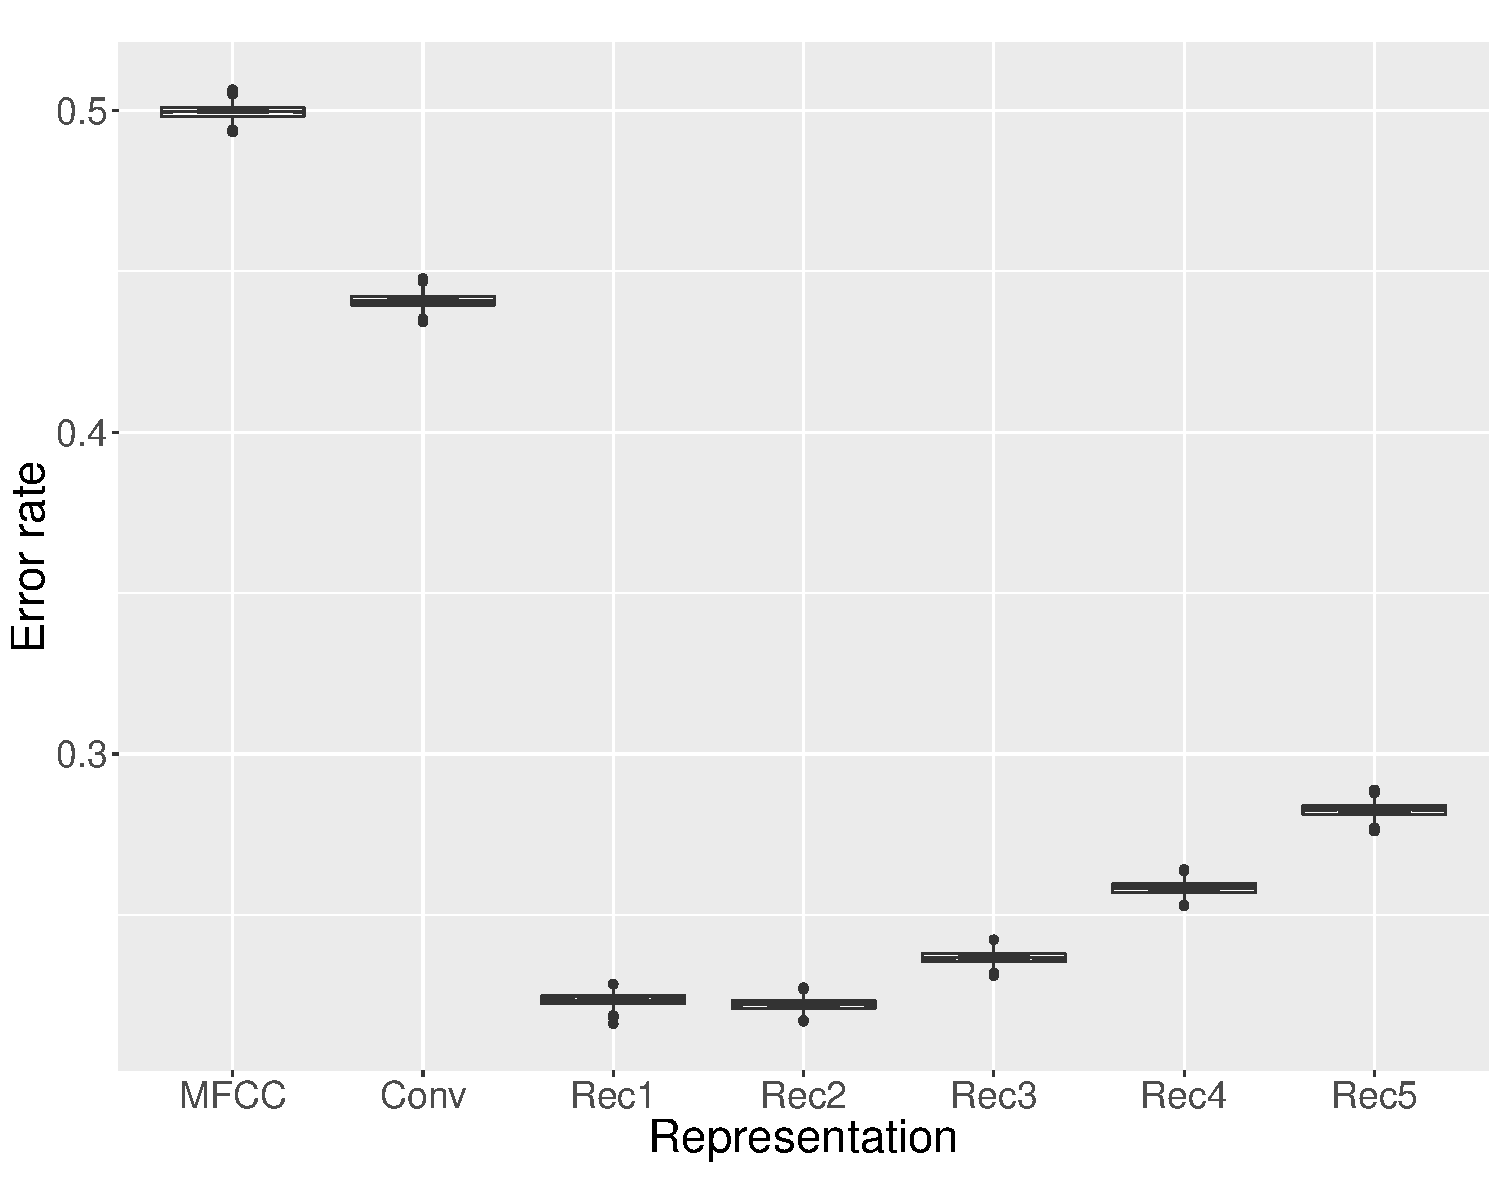
\includegraphics[scale=0.3]{figures/decode.pdf}
  \vspace{-1cm}
     \caption{Accuracy of phoneme decoding with input MFCC features
       and COCO~Speech model activations. The boxplot shows error rates
       bootstrapped with 1000 resamples.}
     \label{fig:decode}
\end{figure}
%% \begin{table}
%%   \centering
%%   \begin{tabular}{l|r}
%%     Representation  & Accuracy  \\\hline
%%     MFCC            & 0.50      \\\hdashline
%%     Convolution     & 0.56      \\
%%     Recurrent 1     & 0.77      \\
%%     Recurrent 2     & 0.78      \\
%%     Recurrent 3     & 0.76      \\
%%     Recurrent 4     & 0.74      \\
%%     Recurrent 5     & 0.72      \\
%%   \end{tabular}
%%   \caption{Accuracy of phoneme decoding with input MFCC features and
%%     COCO~Speech model activations.}
%%   \label{tab:decode}
%% \end{table}
%% ('mfcc', 0.49870657476692304)
%% ('conv', 0.55728398062466367)
%% (0, 0.77430163718120104)
%% (1, 0.77633292244657026)
%% (2, 0.76174933592597094)
%% (3, 0.74003020885779269)
%% (4, 0.71567214708588689)


\subsection{Phoneme discrimination}
\label{sec:abx}

\citet{schatz2013evaluating} propose a framework for evaluating speech features learned in an 
unsupervised setup that does not depend on phonetically labeled data. They propose a set of 
tasks called Minimal-Pair ABX tasks that allow to make linguistically precise comparisons 
between syllable pairs that only differ by one phoneme. They use variants of this task to study 
phoneme discrimination across talkers and phonetic contexts as well as talker discrimination 
across phonemes.

Here we evaluate the COCO~Speech model on the {\it Phoneme across Context} (PaC) task of 
\citet{schatz2013evaluating}. This task consists of presenting a series of equal-length tuples 
$(A, B, X)$ to the model, where $A$ and $B$ differ by one phoneme (either a vowel 
or a consonant), as do $B$ and $X$, but $A$ and $X$ are not minimal pairs.  For example, 
in the tuple ({\it be} /bi/, {\it me} /mi/, {\it my} /\textipa{maI}/),
the task is to identify which of the two syllables /bi/ or /mi/ is closer to /\textipa{maI}/.  The goal is to 
measure context invariance in phoneme discrimination by evaluating how often the model 
recognizes $X$ as the syllable closer to $B$ than to $A$.

\begin{table}
 \centering
 \caption{Accuracy of choosing the correct target in an ABX task using different 
 representations.}
 \label{tab:abx}
 \vspace{.2cm}
 \begin{tabular}{lr}
   \toprule
 { Representation} & {Accuracy} \\
 \midrule
 MFCC &  0.72 \\
 Convolutional & 0.73 \\
 Recurrent 1 &  0.83 \\
 Recurrent 2 &  0.84 \\
 Recurrent 3 &  0.80 \\
 Recurrent 4 &  0.77 \\
 Recurrent 5 &  0.75 \\
 Embeddings  &  0.67 \\
 \bottomrule
 \end{tabular}
 \end{table}


We used a list of all attested consonant-vowel (CV) syllables of American English according to 
the syllabification method described in \citet{Gorman2013}. We excluded the ones which could 
not be unambiguously represented using English spelling for input to the TTS system 
(e.g.\ /\textipa{baU}/). We then compiled a list of all possible $(A, B, X)$ tuples from this list 
where $(A,B)$ and $(B,X)$ are minimal pairs, but $(A,X)$ are not. 
This resulted in 34,288 tuples in total. For each tuple, we measure 
$\mathrm{sign}(\mathrm{dist}(A,X) - \mathrm{dist}(B,X))$, where $\mathrm{dist}(i,j)$ is the 
euclidean distance between the vector 
representations of syllables $i$ and $j$. These representations are either the audio feature 
vectors or the layer activation vectors. A positive value for a tuple means that the model has 
correctly discriminated the phonemes that are shared or different across the syllables.

Table~\ref{tab:abx} shows the discrimination accuracy in this task using various representations. 
The pattern is similar to what we observed in the phoneme identification task: best accuracy is 
achieved using representation vectors from recurrent layers 1 and 2, and it drops as we move 
further up in the model. The accuracy is lowest when final embedding features are used for this task. 




\begin{figure}[t]
  \centering
  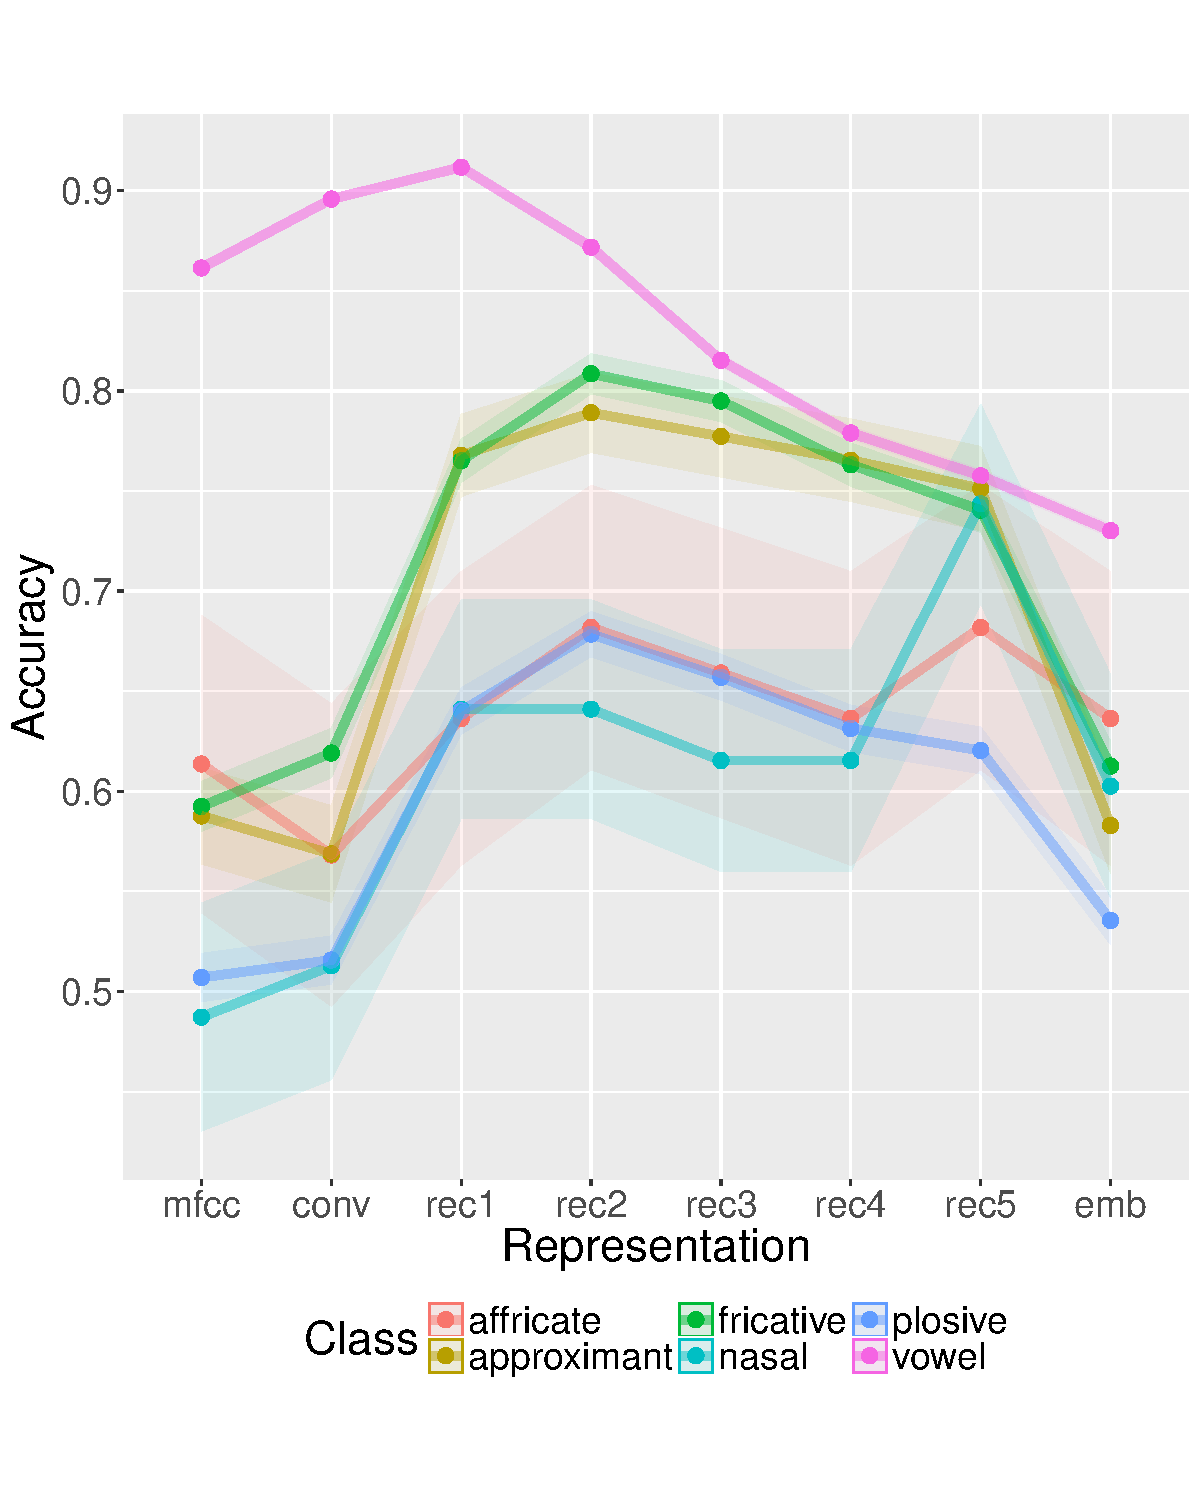
\includegraphics[scale=0.3]{figures/abx_cv_same.pdf}
  \caption{Accuracies for the ABX CV task for the cases where the target
    and the distractor belong to the same phoneme class. Shaded area
    extends $\pm1$ standard error from the mean.}
  \label{fig:abx_cv_same}
\end{figure}

However, the PaC task is most meaningful and challenging where the target and the distractor 
phonemes belong to the same phoneme class. Figure~\ref{fig:abx_cv_same} shows the 
accuracies for this subset of cases, broken down by class.
%
As can be seen, the model can discriminate between phonemes with high accuracy across all 
the layers, and the layer activations are more informative for this task than the MFCC features. 
Again, most phoneme classes seem to be represented more accurately in the lower layers (1--3), and the performance of the model in this task drops as we move towards higher hidden layers. There are also clear differences in the pattern of discriminability for the phoneme classes. The vowels are especially easy to tell apart, but accuracy on vowels drops most acutely in the higher layers. Meanwhile the accuracy on fricatives and approximants starts low, but improves rapidly and peaks around recurrent layer~2. 
The somewhat erratic pattern for nasals and affricates is most likely due to small sample size for these classes, as evident from the wide standard error. 

\subsection{Organization of phonemes}
\label{sec:organization}

In this section we take a closer look at the underlying organization
of phonemes in the model.  Our experiment is inspired by 
\citet{khalighinejad2017dynamic} who study how
the speech signal is represented in the brain at different stages of
the auditory pathway by collecting and analyzing electroencephalography 
responses from participants listening to continuous speech, and show that brain
responses to different phoneme categories turn out to be organized by
phonetic features. 
%They compared the patterns of phoneme
%similarity in the neural responses and the acoustic signals and
%demonstrated that acoustic distinctions of phonemes are reflected in
%the corresponding neural data.

%{\it I assume most of the following paragraph will move to introduction or related work, but I keep it here 
%for now to motivate the experiment. Also most of the content is copied from their paper, so we need to 
%rewrite the text.}
%
%To study how the speech signal is represented in the brain at different stages of the auditory pathway, 
%\cite{khalighinejad2017dynamic} collected electroencephalography responses to continuous speech by 
%obtaining the time-locked responses to phoneme instances (phoneme-related potential), and showed 
%that responses to different phoneme categories are organized by phonetic features. In addition, they 
%compared the patterns of phoneme similarity in the neural responses and the acoustic signals which 
%showed a repetitive appearance of acoustic distinctions of phonemes in the neural data. Their analysis 
%of the phonetic and speaker information in neural activations revealed that different time intervals jointly 
%encode the acoustic similarity of both phonetic and speaker categories. 

%Here we present a simulation of the study of \cite{khalighinejad2017dynamic} by analyzing the hidden 
%layer activations of our model in response to each phoneme in the input, and compare them to the 
%MFCC representations of these phonemes in the speech signal. 
%
%The phoneme activations in each layer, which can be thought as the model's equivalent to the phoneme-
%related potentials, and are calculated as the hidden layer activations averaged over the duration of the 
%phoneme token in the input. The average input vectors are similarly calculated as the MFCC vectors 
%averaged over the time course of the articulation of the phoneme token. Each phoneme type is 
%represented by the average input vector of all its instances in the validation set, and the average 
%activation vector of all its instances for each hidden layer in the model.
%
%%\subsubsection{Correlation with audio representations}
%
%Following \cite{khalighinejad2017dynamic}, we generated a distance matrix for every pair of phonemes 
%by calculating the euclidean distance between the phoneme pair's activation vectors for each layer 
%separately. Similarly, we calculated the distance matrix for the audio vectors of all phoneme pairs in our 
%data. We then calculated the Pearson correlations between the lower triangular part the audio distance 
%matrix and each of activation distance matrix for each layer. 
%\todo{Check that this is what we are doing.}
%>>>>>>> 5719ea4ce48084d7f0d6f9416d2c278836afbc8f



\begin{figure}[t]
  \centering
  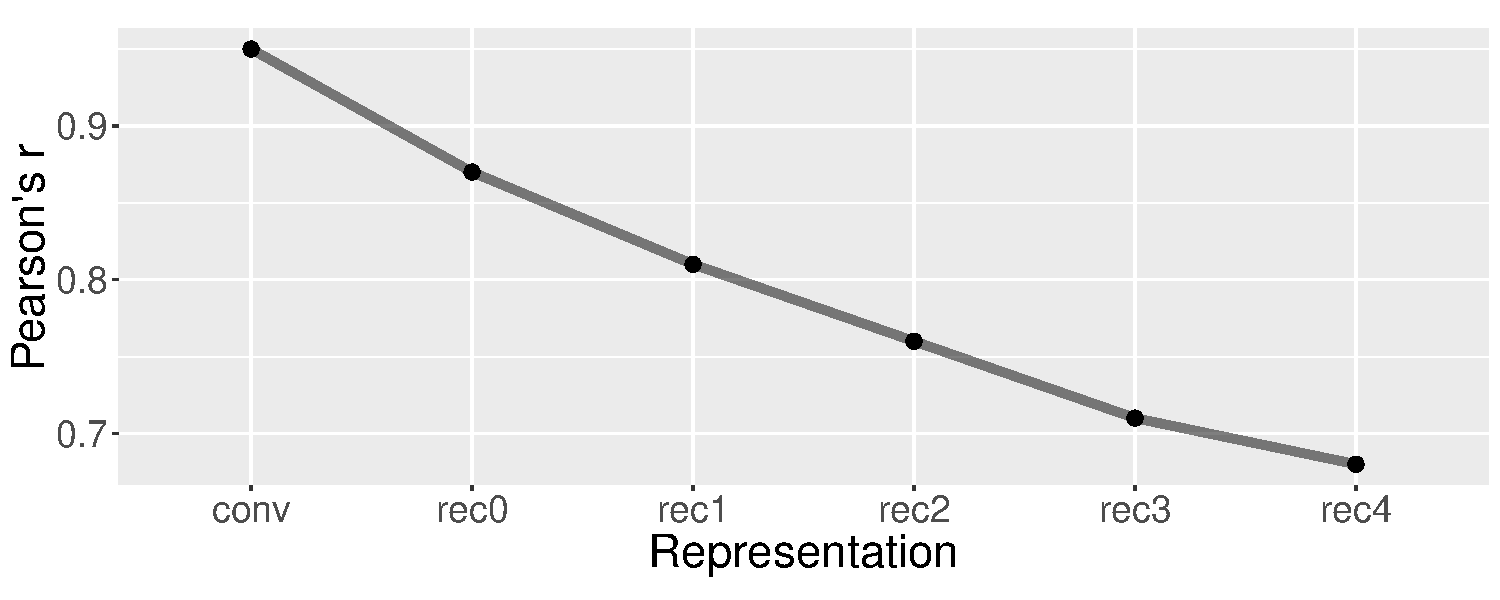
\includegraphics[scale=0.28]{figures/correlation_mfcc.pdf}
  \caption{Pearson's correlation coefficients $r$ between the distance matrix of MFCCs and distance matrices on activation vectors.}
  \label{fig:correlation}
\end{figure}


% Convolutional & 0.95 \\
% Layer 1 &  0.87 \\
% Layer 2 &  0.81 \\
% Layer 3 &  0.76 \\
% Layer 4 &  0.71 \\
% Layer 5 &  0.68 \\



We carry out an analogous experiment by analyzing the hidden layer activations of our model in 
response to each phoneme in the input. First, we generated a distance matrix 
for every pair of phonemes by calculating the Euclidean distance between the 
phoneme pair's activation vectors for each layer separately, as well as a 
distance matrix for all phoneme pairs based on their MFCC features. Similar to 
what \citet{khalighinejad2017dynamic} report,  we observe that the phoneme 
activations on all layers significantly correlate with the phoneme representations 
in the speech signal, and these correlations are strongest for 
the lower layers of the model. Figure~\ref{fig:correlation} shows the results.

%The phoneme activations in each layer, which can be thought as the model's 
%equivalent to the phoneme-
%related potentials, and are calculated as the hidden layer activations 
%averaged over the duration of the 
%phoneme token in the input. The average input vectors are similarly 
%calculated as the MFCC vectors 
%averaged over the time course of the articulation of the phoneme token. Each 
%phoneme type is 
%represented by the average input vector of all its instances in the validation 
%set, and the average 
%activation vector of all its instances for each hidden layer in the model.
%
%\subsubsection{Correlation with audio representations}


%\subsubsection{Organization of phonemes}
%\label{sec:clustering}

%\begin{table*}
%\caption{Evaluation of phoneme clusters based on audio features and layer 
%activations.}
%\label{tab:clustering}
%\begin{center}
%\begin{tabular}{c|c|c|c|c}
%&	{\bf Rand Index}& {\bf Homogeneity} & {\bf Completeness} & {\bf V-
%measure} \\
%\hline
%Audio features		& 0.27		& 0.59		& 0.52		& 0.55 \\
%Activations layer 0	& 0.23		& 0.47		& 0.45		& 0.46 \\
%Activations layer 1	& 0.16		& 0.47		& 0.45		& 0.46 \\
%Activations layer 2	& 0.16		& 0.47		& 0.45		& 0.46 \\
%Activations layer 3	& 0.15		& 0.43		& 0.48		& 0.45 \\
%Activations layer 4	& 0.15		& 0.43		& 0.48		& 0.45 \\
%\hline
%\end{tabular}
%\end{center}
%\end{table*}

%phone mode: short	activation mode: avg
%
%Clustering		Rand Index	Homogeneity	Completeness	V-measure
%Audio features	        0.27		0.59		0.52		0.55
%Conv. activations	0.12		0.44		0.40		0.42
%Activations layer 0	0.23		0.47		0.45		0.46
%Activations layer 1	0.16		0.47		0.45		0.46
%Activations layer 2	0.16		0.47		0.45		0.46
%Activations layer 3	0.15		0.43		0.48		0.45
%Activations layer 4	0.15		0.43		0.48		0.45
%
%---------
%
%phone mode: long	activation mode: avg
%
%Clustering		Rand Index	Homogeneity	Completeness	V-measure
%Audio features		0.18		0.45		0.42		0.44
%Conv. activations	0.20		0.43		0.41		0.42
%Activations layer 0	0.16		0.43		0.40		0.41
%Activations layer 1	0.11		0.39		0.39		0.39
%Activations layer 2	0.11		0.40		0.38		0.39
%Activations layer 3	0.06		0.33		0.38		0.35
%Activations layer 4	0.06		0.28		0.32		0.30

%% \begin{figure*}[t]
%%   \centering
%%   \includegraphics[scale=0.37]{figures/audio.png}
%% \caption{Hierarchical clustering of phoneme audio vectors.}
%% \label{fig:cluster-audio}
%% \end{figure*}
%% \begin{figure*}[t]
%%   \centering
%%   \includegraphics[scale=0.37]{figures/activation4.png}
%% \caption{Hierarchical clustering of phoneme activation vectors on the last 
%%  hidden layer.}
%% \label{fig:cluster-l4}
%% \end{figure*}
We then performed agglomerative hierarchical clustering on phoneme type MFCC and 
activation vectors, using Euclidean distance as the distance metric and the Ward linkage criterion \citep{ward1963hierarchical}.
%We compared the class labels extracted from the clustering tree to a set of 
%manually-annotated gold-standard labels for phoneme categories. 
%Table~\ref{tab:clustering} shows the clustering results.
Figure~\ref{fig:cluster-l0} shows the clustering results for the activation vectors
on the first hidden layer. The leaf nodes are color-coded according to phoneme classes as specified in Table~\ref{tab:phoneme-list}. There is substantial degree of matching between the classes and the structure of the hierarchy, but also some mixing between rounded back vowels and voiced plosives /b/ and /g/, which share articulatory features such as lip movement or tongue position. 
\begin{figure}[ht]
  \centering
  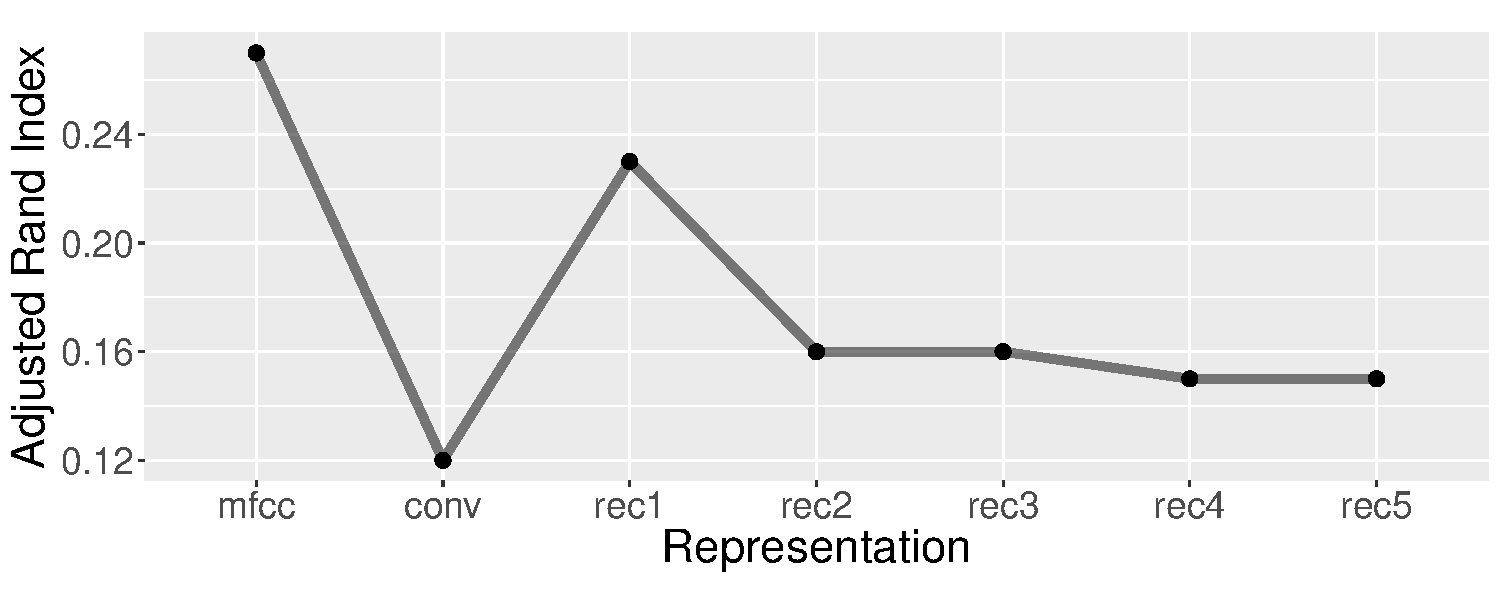
\includegraphics[scale=0.3]{figures/hier_ari.pdf}
  \caption{Adjusted Rand Index for the comparison of the phoneme type hierarchy induced from representations against phoneme classes.}
  \label{fig:hier_ari}
\end{figure}

We measured the adjusted Rand Index for the match between the
hierarchy induced from each representation against phoneme classes,
which were obtained by cutting the tree to divide the cluster into the
same number of classes as there are phoneme classes. There is a notable drop between the match from MFCC to the activation of the convolutional layer. We suspect this may be explained by the loss of information caused by averaging over phoneme instances combined with the lower temporal resolution of the activations compared to MFCC. The match improves markedly at recurrent layer~1.


\begin{figure*}[t]
  \centering
  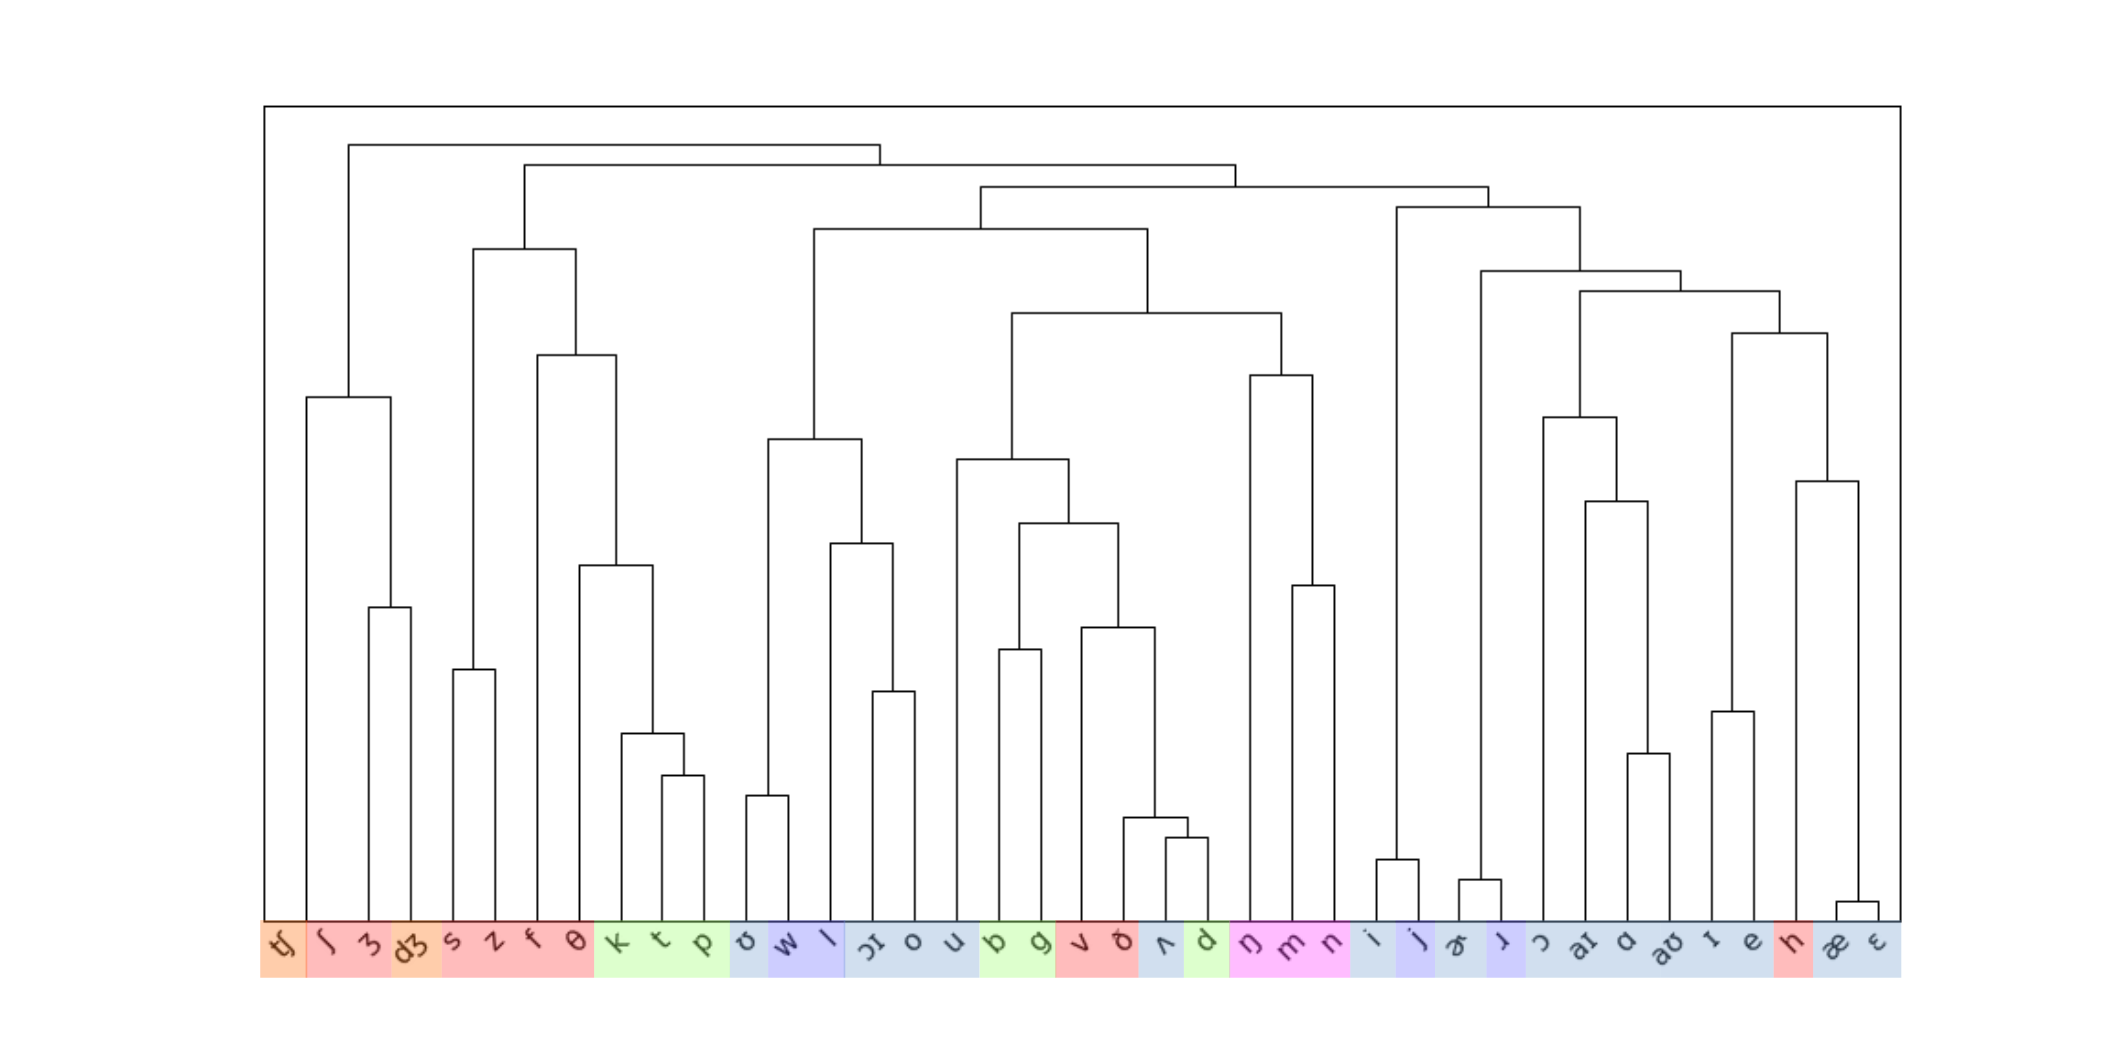
\includegraphics[scale=0.45]{figures/color-coded-activation0.png}
\caption{Hierarchical clustering of phoneme activation vectors on the first 
hidden layer.}
\label{fig:cluster-l0}
\end{figure*}




\subsection{Synonym discrimination}
\label{sec:synonym}

Next we simulate the task of distinguishing between pairs of synonyms, i.e.\ words with different acoustic forms but the same meaning. With a representation encoding phonological form, our expectation is that the task would be easy; in contrast, with a representation which is invariant to phonological form in order to encode meaning, the task would be hard. 

We generate a list of synonyms for each noun, verb and adjective in the validation data using Wordnet \citep{miller1995wordnet} synset membership as a criterion. Out of these generated word pairs, we select synonyms for the experiment based on the following criteria:
\begin{itemize}
\item both forms clearly are synonyms in the sense that one word can be replaced by the other without changing the meaning of a sentence,
\item both forms appear more than 20 times in the validation data, 
\item the words differ clearly in form (i.e. they are not simply variant spellings like {\it donut/doughnut, grey/gray}),
\item the more frequent form constitutes less than 95\% of the occurrences.
\end{itemize}
This gives us 2 verb, 2 adjective and 21 noun pairs.

For each synonym pair, we select the sentences in the validation set in which one of the two forms appears. We use the POS-tagging feature of NLTK \citep{bird2006nltk} to ensure that only those sentences are selected in which the word appears in the correct word category (e.g.\ {\it play} and {\it show} are synonyms when used as nouns, but not when used as verbs). We then generate spoken utterances in which the original word is replaced by its synonym, resulting in the same amount of utterances for both words of each synonym pair.

\begin{figure}[!ht]
  \centering
  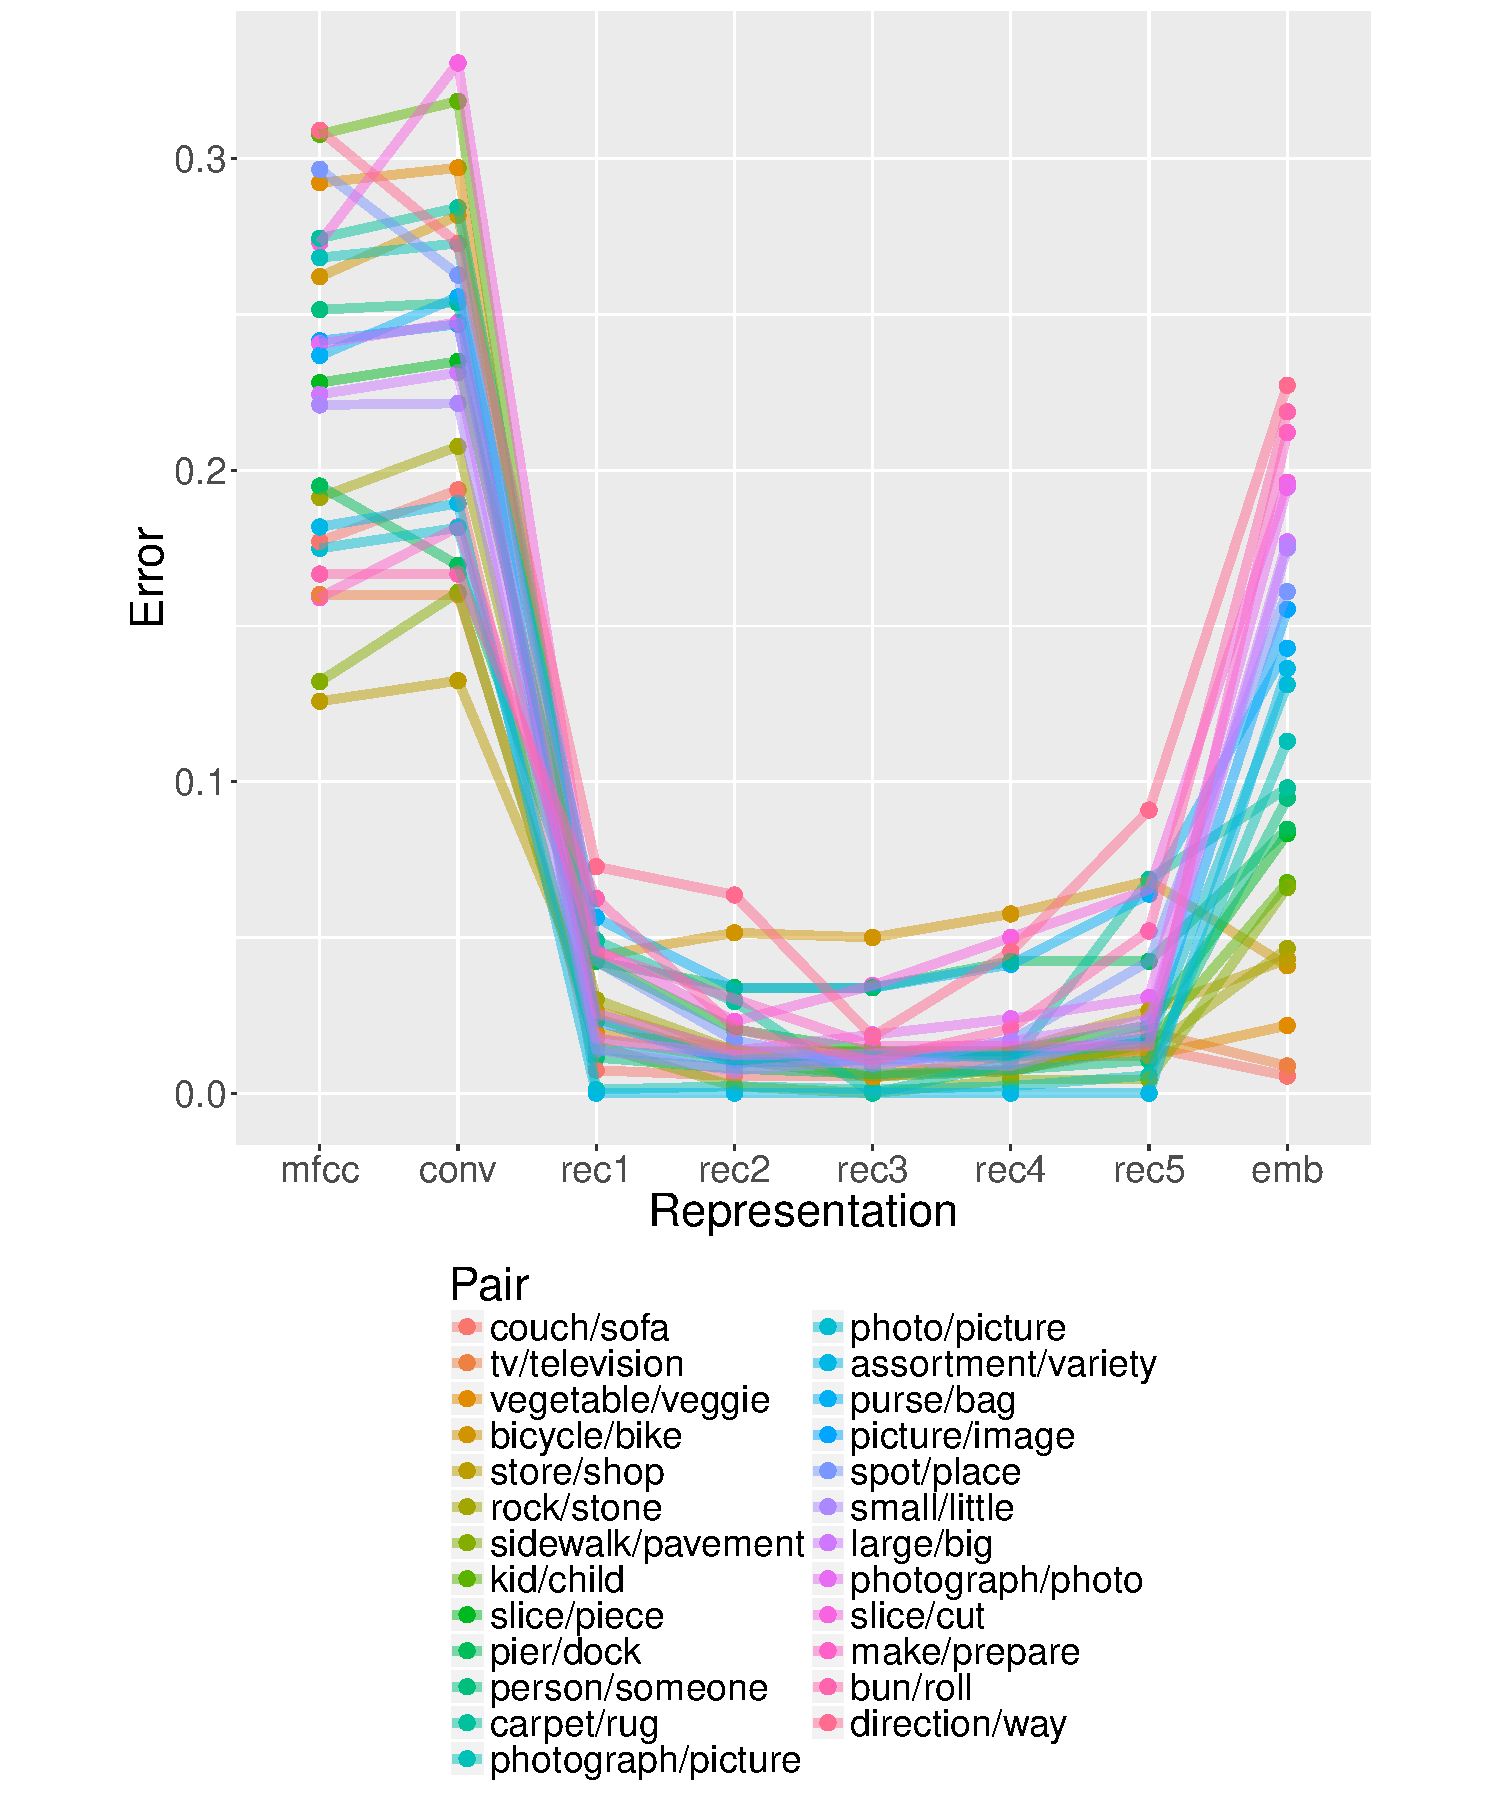
\includegraphics[scale=0.3]{figures/synonym.pdf}
  \caption{Synonym discrimination error rates, per representation and synonym pair.}
  \label{fig:synonyms}
\end{figure}


For each pair we generate a binary classification task using the MFCC features, the average activations in the convolutional layer, the average unit activations per recurrent layer, and the sentence embeddings as input features. For every type of input, we run 10-fold cross validation using Logistic Regression to predict which of the two words the utterance contains.  We used an average of 672 (minimum 96; maximum 2282) utterances for training the classifiers.

Figure~\ref{fig:synonyms} shows the error rate in this classification task for each layer and each synonym pair. Recurrent layer activations are more informative for this task than MFCC features or activations of the convolutional layer.  Across all the recurrent layers the error rate is small, showing that some form of phonological information is present throughout this part of the model. However, sentence embeddings give relatively high error rates suggesting that the attention layer acts to focus on semantic information and to filter out much of phonological form.


